% ============================================================================
% Paper 6 -- integrated from papers/_FGCS____DIGITA_25_extended__camera_ready_(1)/cas-dc-template.tex (front
% matter transcribed from the cas-dc \title/\tnotetext/\author/\affiliation, abstract, highlights and keywords;
% body converted mechanically, see the integration report). The source contains \credit{} commands but
% \printcredits is commented out, so no CRediT statement is printed (as in the source).
% ============================================================================
\section{A Knowledge Graph-Driven Framework for Deploying AI-Powered Patient Digital Twins}
\label{sec:paper6}

\noindent This section contains the article~\cite{MARFOGLIA2026108380}.

\paragraph{Authors.}
Alberto Marfoglia\textsuperscript{1,*}, Christian D'Errico\textsuperscript{1}, Sabato Mellone\textsuperscript{2}, Antonella Carbonaro\textsuperscript{1}

{\raggedright % layout: ragged-right metadata block
\noindent\textsuperscript{1}Dept. of Computer Science and Engineering - DISI, University of Bologna, Cesena, Italy\\
\textsuperscript{2}Dept. of Electrical, Electronic and Information - DEI, Engineering ``Guglielmo Marconi'', Bologna, Italy\\
\textsuperscript{*}Corresponding author: Alberto Marfoglia (alberto.marfoglia2@unibo.it)\\
E-mail addresses: alberto.marfoglia2@unibo.it (A. Marfoglia), christian.derrico2@unibo.it (C. D'Errico), sabato.mellone@unibo.it (S. Mellone), antonella.carbonaro@unibo.it (A. Carbonaro).\\
ORCID: \url{https://orcid.org/0009-0000-5857-2376} (A. Marfoglia), \url{https://orcid.org/0009-0002-5784-0492} (C. D'Errico), \url{https://orcid.org/0000-0001-7688-0188} (S. Mellone), \url{https://orcid.org/0000-0002-3890-4852} (A. Carbonaro). \\
Future Generation Computer Systems 180 (2026) 108380. \url{https://doi.org/10.1016/j.future.2026.108380}. Received 20 May 2025; Received in revised form 23 October 2025; Accepted 16 January 2026; Available online 20 January 2026.\\ 0167-739X/\textcopyright{} 2026 The Author(s). Published by Elsevier B.V. This is an open access article under the CC BY license (\url{http://creativecommons.org/licenses/by/4.0/}). 
\par}

\subsection*{Abstract}

Background: The healthcare sector faces diverse challenges, including poor interoperability and a lack of personalized approaches, which limit patient outcomes. Ineffective data exchange and one-size-fits-all treatments fail to meet individual needs. Emerging technologies like digital twins (DTs), the semantic web, and AI show promise in tackling these obstacles. For this reason, we introduced CONNECTED, a conceptual multi-level framework that combines these techniques to deploy general-purpose patient DTs.
%
Objective: This study assesses CONNECTED's comprehensiveness, applicability, and utility for developing intelligent, personalized healthcare applications. Specifically, we deliver a preliminary version of the framework to predict future patient states and demonstrate its automation benefits in deploying semantically enriched, AI-powered patient DTs.
%
Methods: We enhanced the CONNECTED architecture by providing a formal definition of DT and modularizing its core functionalities into microservices—Properties, State, Capabilities, and Manifest. The Manifest service facilitates AI model integration through the Model Interface Manifest Ontology (MIMO), enabling automatic data-to-model binding via a reasoner. Using the HeartBeatKG quality assessment tool, we validated MIMO and tested the internal logic by integrating a well-established stroke-risk model.
%
Results: Our implementation comprehends: (1) deploying a FHIR-compliant, patient-centric API for clinical history access, real-time monitoring, and predictive simulation; (2) publishing MIMO; (3) establishing the Manifest protocol for seamless, general-purpose AI model integration tailored to individual patient profiles; and (4) a proof-of-concept benchmarking application comparing multiple stroke risk classifiers.
%
Conclusion: CONNECTED establishes a flexible, scalable foundation for interoperable semantic patient DTs. Automation reduces technical overhead and enables users to focus on delivering personalized, insight-driven care.

\subsection*{Highlights}

\begin{itemize}
\item Enable patient digital twin deployment via a knowledge-driven, modular framework
\item Provide clinical data access and simulation through a FHIR-compliant API
\item Publish MIMO ontology to standardize and increase transparency of AI model interfaces
\item Automate AI model integration using a manifest-based binding protocol
\item Benchmark stroke risk models with real-time, time-aware clinical data streams
\end{itemize}

\paragraph{Keywords:} Digital Twins; Healthcare; Knowledge Graphs; Machine Learning Models; Pervasive Computing; Semantic Web; Personalized Medicine; Predictive Analytics

\subsection{Introduction}~\label{paper6_introduction}
The ongoing digital transformation of healthcare is reshaping how care is delivered, driven by the increasing need to integrate heterogeneous, real-time data streams and provide more personalized, patient-centered services \cite{engstrom_impact_2023,amri_data-driven_2023}. These advancements promise improved precision in diagnosis and treatment, reduced side effects, and greater patient empowerment \cite{engstrom_impact_2023,cailleaux_fused_2021}.
%%%% CHANGED: 
%However, realizing this potential remains challenging due to fragmented data sources, a lack of interoperability, and the absence of scalable architectures that support seamless communication across systems \cite{mumtaz_current_2023}.
%%%% TO:
However, the full realization of these advancements remains constrained by fragmented data ecosystems, limited interoperability, and the absence of scalable, knowledge-driven architectures capable of unifying data and services across institutions~\cite{mumtaz_current_2023}.

Digital Twins (DTs), virtual replicas that continuously mirror the status and behavior of physical systems, are gaining traction in healthcare as tools for real-time patient monitoring \cite{johnson_digital_2024}, personalized treatment planning \cite{vallee_digital_2023}, and optimizing clinical operations \cite{sun_digital_2023}. Yet, despite their promise, current healthcare DTs face several limitations. These include the difficulty of multi-scale modeling, limited access to high-quality and standardized clinical data for validation \cite{arcobelli2024fhir,marfoglia_towards_2025}, and rigid, vertically designed architectures that inhibit interoperability and reuse across settings \cite{9325551_ricci}.
%%%% CHANGED:
%%%% TO:
Therefore, enabling interoperable, semantically enriched, and AI-augmented DT frameworks is essential to realize the vision of continuous, personalized, and predictive healthcare.

Concurrently, Artificial Intelligence (AI) and the Internet of Things (IoT) are automating time-intensive clinical tasks, particularly in domains such as precision imaging \cite{johnson_precision_2021}. While AI is expected to become central in advancing integrated, data-driven healthcare systems \cite{gupta_artificial_2021}, its effectiveness depends heavily on high-quality, multi-modal data and rigorous real-world validation. In addition, using AI in clinical decision-making raises ethical challenges related to transparency, explainability, and accountability \cite{sun_ai_2023}.

Knowledge representation is another cornerstone of intelligent healthcare systems. Among the most effective tools in this area are knowledge graphs (KGs), which structure complex, interconnected data to improve integration, reasoning, and scalability \cite{peng_knowledge_2023}. In healthcare, KGs help bridge data silos and enhance decision support by facilitating semantic interoperability and trust in machine-generated insights \cite{peng_knowledge_2023,abu-salih_healthcare_2023}.

To address these architectural and integration challenges while unifying the strengths of DTs, AI, and KGs, we propose CONNECTED (COmpreheNsive and staNdardized hEalth-Care plaTforms to collEct and harmonize clinical Data) \cite{10.3389/fdgth.2023.1322428_carbonaro_connected}, a multi-level framework for deploying general-purpose patient DTs following a DTs-as-a-service (DTaaS) approach. CONNECTED is designed to aggregate clinical data across sources, support real-time monitoring, and ensure interoperability through semantic web technologies. In its original conception, CONNECTED enabled patient DTs to store structured clinical histories as KGs and provide dynamic status updates on demand \cite{10.3389/fdgth.2023.1322428_carbonaro_connected}.

We then extended CONNECTED by equipping DTs with predictive simulation capabilities powered by AI models \cite{marfoglia_2024_mimo}. To enable their seamless integration, we designed the Manifest protocol. Each model is accompanied by an RDF machine-readable formal description, called  Manifest, which specifies the functional requirements needed to execute it, such as input, output, location, and runtime constraints. Once uploaded into the framework, each Manifest can be linked to patient-specific DTs via the Capability abstraction defined in CONNECTED's DT Layer.

The Manifest protocol enables automatic integration of AI models, regardless of algorithmic implementation, communication protocol, or hosting environment. The Capability abstraction further enhances model potential by tailoring general-purpose models to the unique characteristics of each patient, thus supporting personalized care. Moreover, because both model interfaces and DT states are represented semantically as KGs, CONNECTED can automatically extract the required patient data, invoke the model with appropriate inputs, and record the outputs as predictive outcomes within the DT. This degree of automation and the CONNECTED API significantly reduces the technical burden on users, allowing them to focus on insight-driven decision-making.

This paper evaluates CONNECTED's comprehensiveness, applicability, and utility for developing intelligent and personalized healthcare applications. We introduce a preliminary implementation designed to forecast patient health trajectories and demonstrate its ability to automate the deployment of semantically enriched, AI-powered DTs. 

Our implementation achieves four key contributions:
\begin{itemize}
    \item A FHIR-compliant, patient-centric API that enables access to clinical histories, real-time monitoring, and predictive simulation;
    \item The publication of the Model Interface Manifest Ontology (MIMO) in the Linked Open Data Cloud (LOD) to support transparent and standards-based model descriptions;
    \item The implementation of the Manifest protocol, enabling automated data-to-model binding and seamless integration of general-purpose AI models into patient DTs;
    \item A proof-of-concept benchmarking application built on the CONNECTED API, enabling the dynamic integration, evaluation, and comparison of multiple stroke risk classifiers. Incoming data streams drive continuous, time-aware model selection and performance ranking.
\end{itemize}
%%%% CHANGED:
% The remainder of this paper is structured as follows. Section~\ref{sec:related_work} surveys related work on healthcare DTs and foundational frameworks, positioning our contributions within the current landscape. Section~\ref{sec:architectural_background} describes the CONNECTED architecture and its core components. Section~\ref{sec:results} presents the core results, including the FHIR-compliant DT API, the MIMO ontology, the implementation of the Manifest protocol for stroke risk classification, and a proof-of-concept benchmarking application. Finally, Section~\ref{sec:discussion} discusses limitations and outlines future research directions.
%%%% TO:
The remainder of this paper is structured as follows. Section~\ref{sec:paper6_related_work} surveys related work on healthcare DTs and foundational frameworks, positioning our contributions within the current landscape. Section~\ref{sec:paper6_architectural_background} presents the CONNECTED architecture, followed by the implementation details in Section~\ref{sec:paper6_implementation}. Section~\ref{sec:paper6_manifest_protocol} describes the Manifest protocol, and Section~\ref{sec:paper6_evaluation} presents our evaluation results. Section~\ref{sec:paper6_discussion} provides a broader discussion of findings and limitations, outlining future research directions.

\subsection{Related Work}~\label{sec:paper6_related_work}
DT frameworks have seen growing interest across multiple domains. However, most existing solutions originate from industrial applications~\cite{wang_mobility_2022}and are not well-suited to the unique challenges of healthcare. These include heterogeneous clinical data integration, adherence to stringent interoperability standards, and the need for patient-centered design. As a result, many general-purpose DT architectures lack the semantic, dynamic, and modular features required for medical applications.
%
%%%% CHANGED:
%\subsection{Healthcare-Specific DT Efforts}
%%%% TO:
\subsubsection{Patient-Centric DT Initiatives}
Several efforts have sought to tailor DTs to clinical use cases. Saxby et al.~\cite{saxby_digital_2023} explored DTs for neuromusculoskeletal modeling, demonstrating their utility for tendon strain analysis and neurorehabilitation. However, their approach lacks standardized mechanisms for data exchange, limiting scalability and integration potential.

In a more patient-specific approach, Rad et al.~\cite{sarani_rad_personalized_2024} present a DT framework for diabetes management using Personal Knowledge Graphs (PKGs). Although their use of FHIR-aligned ontologies supports data integration and real-time decision-making, they do not offer a patient DT formal definition or provide reusable implementation artifacts, limiting reproducibility.

Similarly, Jameil et al.~\cite{jameil_digital_2025} integrate IoT and hybrid machine learning for anomaly detection in real-time monitoring. Despite technical maturity, their work conflates DT and AI components and does not propose a modular, generalizable framework for semantic model integration.
%
%%%% CHANGED:
%\subsection{Semantic and Knowledge-Driven Architectures}
%%%% TO:
\subsubsection{Knowledge-Driven Architectures}
KGs are increasingly leveraged to enhance semantic interoperability and reasoning in DTs. Jinzhi et al.~\cite{jinzhi_exploring_2022} propose a KG-based DT framework with reasoning capabilities to forecast future states. However, it lacks healthcare-specific adaptability and contextualization.

Sahlab et al.~\cite{sahlab_knowledge_2021} introduce a KG-enhanced DT framework for Cyber-Physical Systems (CPS), supporting internal linking, error detection, and semantic querying. While rich in knowledge processing, the framework struggles with integrating digital artifacts and lacks standard data formats, making AI model integration cumbersome.

Lee et al.~\cite{lee_digital_2025} explore the construction of PKGs using SNOMED CT and LOINC to support AI-driven healthcare services. Their design emphasizes longitudinal patient records but lacks temporal reasoning capabilities and a clear DT formalization, hindering real-time adaptability and personalization.
%
\subsubsection{Foundational Frameworks}
At a more abstract level, Angelelli et al.~\cite{pellegrino_conceptual_2025} offer a conceptual framework that identifies 11 key dimensions for DT evaluation in healthcare, including modularity and interoperability. While useful as a design compass, it lacks empirical validation and does not provide implementation strategies or code artifacts.

Ricci et al.~\cite{9325551_ricci} propose a service-oriented architecture using horizontally layered, API-driven components to improve composability and interoperability. While conceptually aligned with modern software principles, their framework remains under-specified in implementation. Specifically, they omit mechanisms for semantic integration, AI model binding, or patient-level personalization—features central to real-world deployment.

Lombardo et al.~\cite{LOMBARDO2024107203} address real-time learning through a DT architecture focused on intelligent location-based services. Although capable of continual adaptation, the system lacks patient-centered care mechanisms and does not leverage semantic representations, limiting its relevance for personalized clinical applications.

\subsubsection{Summary and Differentiation}
Across prior work, a recurring gap emerges between conceptual richness and implementation maturity. Many frameworks offer theoretical contributions or single-purpose prototypes, but fall short in three critical areas:
%
\begin{enumerate}
    \item A formal definition of patient-specific DTs: specifying their responsibilities and functional boundaries. For example, what types of patient data can be retrieved and observed? What kinds of simulations can be performed? DTs remain abstract and difficult to standardize or operationalize without such a definition.
    \item Semantic-level interoperability: the ability to automatically interpret and integrate data across heterogeneous systems using shared ontologies and standard vocabularies. A key challenge is to collect, harmonize, and store vast amounts of clinical data while preserving, and ideally enriching, its semantic meaning.
    \item Modular integration of AI models: enabling algorithms to be seamlessly connected to patient data in a plug-and-play fashion, supporting personalized and predictive care with minimal manual configuration. A robust framework should provide an abstraction layer between AI models and DT functionalities to support continuous integration, model comparison, and replacement. This facilitates dynamic evaluation and selection of the most appropriate model for predicting specific patient trajectories.
\end{enumerate}
%
CONNECTED addresses these challenges by offering both a conceptual and technical solution. Conceptually, it organizes functionalities into a layered architecture and defines a patient-oriented DT model. Technically, it delivers:
%
\begin{itemize}
    \item A microservice-based architecture that exposes DT functionalities through a FHIR-compliant RESTful API, enabling access to clinical histories, observation of current patient states, and execution of predictive simulations;
    \item The Manifest protocol and MIMO to describe, bind, and execute AI models in a transparent, reusable, and interoperable manner;
    \item The use of semantic web technologies to harmonize and enrich patient data and AI model interfaces. This allows automatic data-to-model matching and ensures consistent knowledge management as the ecosystem evolves.
\end{itemize}
%
Through this combination, CONNECTED offers a generalizable and scalable foundation for intelligent, patient-centered DTs in healthcare, reducing technical overhead while overcoming long-standing barriers to standardization, semantic interoperability, and modular AI integration.

%%%% CHANGED:
% \section{Methods}~\label{sec:methods}
%%%% TO:
\subsection{Architectural background}~\label{sec:paper6_architectural_background}
%%%% CHANGED:
%This section presents the architectural and methodological foundations underpinning the CONNECTED framework.
%It aims to address key challenges in real-time data integration, semantic interoperability, and intelligent service orchestration by abstracting the complexity of physical systems and offering a uniform digital representation of patients. Inspired by the cyber–physical abstraction principles and the DTaaS paradigm, CONNECTED structures its components to support scalable, interoperable, and domain-agnostic applications.

% The following subsections outline the design principles, system architecture, and semantic technologies that constitute the core of the CONNECTED platform.
%%%% TO:
This section provides a concise recap of the CONNECTED architecture and the DT conceptual model. For a comprehensive extended discussion of the original design principles and motivation, the reader is referred to our prior works~\cite{10.3389/fdgth.2023.1322428_carbonaro_connected,marfoglia_connected_2025}.

%%%% CHANGED:
% \subsection{From Data Sources to Services: A Multi-Layered Approach}
%%%% TO:
\subsubsection{Multi-layer Architecture}
This CONNECTED framework introduces a multi-layer architecture (Figure~\ref{paper6_fig1}) comprising four key layers: \textit{Source}, \textit{Standard}, \textit{Digital Twin}, and \textit{Application}, each responsible for a specific function within the system. The framework employs a modular, layered structure to manage data flows and decouple services, providing flexibility and robustness in handling heterogeneous data sources and dynamic healthcare requirements. Each framework's layer plays a critical role in ensuring the smooth flow of data and functionality between physical systems and high-level applications.
%
\begin{figure}
    \centering
    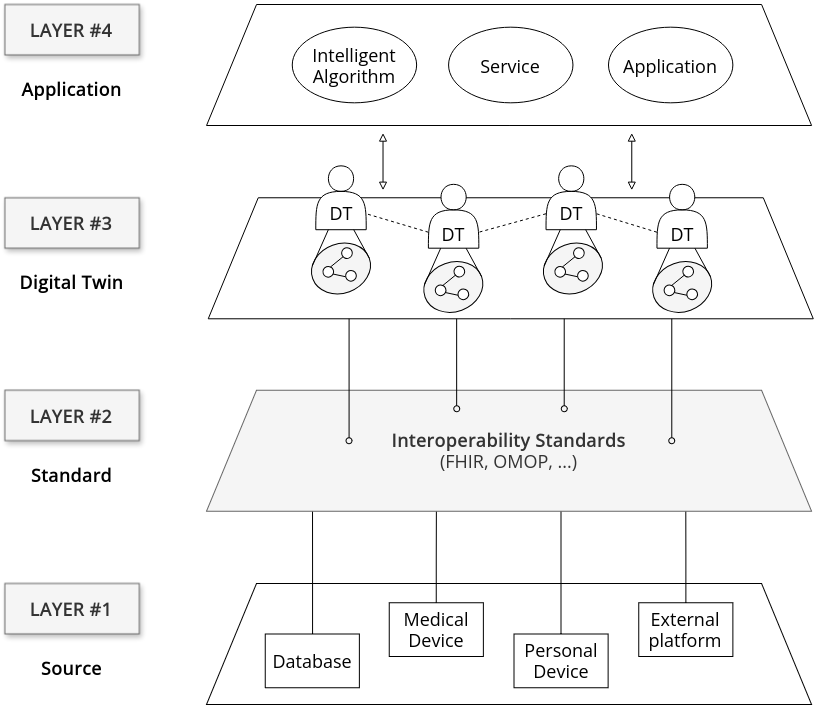
\includegraphics[width=1\linewidth]{figures/paper6/fig1.png}
    \caption{Diagram of the 4-tier architecture setup: data from the sources, structured with FHIR resources, are used to update the DTs' states, enabling functionality for applications and services in the highest layer.}\label{paper6_fig1}
\end{figure}
%
The Source Layer collects data in real-time from a wide array of devices, including medical and IoT devices, smartphones, and healthcare platforms. This layer functions as a data funnel, handling varying data volumes, formats, and protocols. It preprocesses the incoming data to ensure it is ready for further processing in the next layer.

The Standard Layer ensures interoperability across heterogeneous systems by adopting well-established healthcare standards such as FHIR. Incoming data is harmonized and transformed into a common format that supports interoperability across different devices and platforms. This layer includes adapters to process data from legacy and proprietary formats, facilitating integration with modern healthcare standards.

At the heart of the framework, the DT Layer creates virtual replicas of physical patients. These DTs enable real-time monitoring, retrieval of clinical history, and predictive analytics. This layer structures the collected data by employing KGs and ontologies to support advanced reasoning and inference, enabling the generation of insights into patient health.

The Application layer hosts applications that interact with the DTs via APIs. These applications range from simple visualization tools to complex decision-support systems that assist clinicians in decision-making. This layer leverages the data and capabilities provided by the DTs to deliver personalized and preventive care services. The API-driven architecture ensures that applications are not tightly coupled to specific DTs, enhancing the system’s flexibility and scalability.
%
%%%% CHANGED:
% \subsection{The Role of the Digital Twin Paradigm}
%%%% TO:
\subsubsection{Digital Twin Model}
The DT paradigm is an abstraction that bridges physical and digital layers of healthcare systems. DTs in CONNECTED are not static replicas, but intelligent, evolving entities that unify data from diverse sources, support semantic reasoning, and expose actionable interfaces for clinical applications. Healthcare data arises from heterogeneous sources (e.g., wearables, medical devices, and hospital systems) using different formats and protocols. The DT Layer abstracts this complexity by harmonizing inputs into a consistent digital representation. This cyber–physical decoupling enables the provision of a uniform abstraction and service level functionality to upper layers. In this way, these latter can focus on analysis and decision-making without needing to manage low-level infrastructural details. 

Each DT operates as an independent service under the DTaaS paradigm, exposing well-defined RESTful APIs to access state, trigger simulations, and retrieve derived insights. This modular design allows applications to interact with DTs in a scalable and reusable way, avoiding domain-specific silos.

Beyond mere data mirroring, each DT maintains a KG that semantically integrates heterogeneous, real-time data with domain ontologies and logical rules. This semantic layer supports reasoning over the patient's condition, enabling the inference of clinical states, risk factors, or behavioral trends, essential for preventive and personalized care.

In our framework, the DT serves as a virtual patient replica, describing the patient’s pathophysiology through three primary components:
\begin{itemize}
    \item \textbf{Properties}: A set of immutable attributes that define the identity and core characteristics of the patient, such as demographic data. By isolating fixed identifiers, Properties ensure consistency across systems, simplify data linkage, and reduce update complexity, supporting long-term traceability.
    \item \textbf{State}: A dynamic, time-sensitive information representing the patient’s evolving condition, including vital signs and clinical observations. The state supports real-time monitoring, which can be retrieved at any point as a historical snapshot. It also supports a shadowing mechanism to remain synchronized with incoming data, ensuring digital fidelity.
    \item \textbf{Capabilities}: A set of virtual operations or simulations the DT can perform, powered by algorithms that process its State and Properties to predict health outcomes or support clinical decisions. Moreover, Capabilities decouple prediction goals from implementation strategies, enabling the definition and comparison of multiple approaches to achieve the same objective.
\end{itemize}
%
\subsection{Platform implementation}\label{sec:paper6_implementation}
The implementation presented in this paper realizes the conceptual architecture summarized in Section~\ref{sec:paper6_architectural_background}. 
%%%% CHANGED:
%%%% TO:
Developing CONNECTED introduces several challenges, many of which fall outside the scope of our research. To address this, we have refined the platform's features based on the following assumptions: (i) The Application Layer can be emulated using a straightforward REST client, such as Postman; (ii) Data from the Source Layer are reliable, conform to the FHIR model, and include the DT's identifier; (iii) Any required data preprocessing is handled directly by the models, and (iv) Communication between the source and higher layers operates on a push-based model. 
%%%% CHANGED:
%These considerations enable us to concentrate on the DT Layer, as its development can contribute novel insights to the scientific community.
%Below we describe the concrete choices, microservice decomposition, and data-flow mechanisms that constitute the platform built for the experiments and validation reported in Section~\ref{sec:results}.
%%%% TO:
These assumptions allow us to focus primarily on the DT Layer, as its design and implementation can contribute novel insights to the scientific community. The following sections describe the concrete implementation choices, microservice decomposition, and data-flow mechanisms that form the basis of the platform used for the experiments and validation discussed in Section~\ref{sec:paper6_evaluation}.
%
%%%% CHANGED:
% \subsection{From Conceptual to a Microservice Implementation}
%%%% TO:
\subsubsection{Microservice Architecture}
The multi-layered structure of CONNECTED, combined with its diverse use cases and evolving requirements, led us to adopt a microservices architecture; a detailed description is provided in~\cite{marfoglia_connected_2025}. This approach improves maintainability by isolating components, minimizes interdependencies between services, and offers the flexibility needed to scale and adapt to future demands. By adhering to the information-hiding principle, each microservice exposes only minimal interfaces, thereby managing the system's complexity. Additionally, microservices avoid shared state or storage, enabling independent deployments and reducing the risk of system-wide failures.

A key challenge in a microservices architecture is defining clear service boundaries. From domain-driven design, services are segmented by business domains rather than specific functionalities. This domain-oriented approach simplifies feature development and integration, making it more cost-effective to introduce new capabilities or combine existing ones, rather than altering established services.

Each microservice follows the hexagonal architecture pattern~\cite{martin2017clean}, decoupling core business logic from external dependencies such as frameworks and libraries. This isolation ensures that DT functionalities remain agnostic to the implementation. By organizing internal modules in this layered, "onion-like" structure, we increase flexibility, streamline collaboration across teams, and simplify the development of unit tests.
%%%% CHANGED:
%%%% TO:
\subsubsection{Digital Twin Layer Services}
The functionalities of the DT Layer are structured into four independent Ktor web services (Figure \ref{paper6_fig2}): Model, Capability, State, and Property. The Manifest service allows the uploading, updating, and deleting of manifests, while the other three provide concrete implementations of the DT conceptualization introduced in the previous subsection. Additionally, we have developed a DT Manager that oversees the addition and modification of DT instances, ensuring the integrity of DT identifiers and maintaining consistency between the State and Capability services. Moreover, the Capabilities service interacts with a MongoDB database to store associations between DT and Manifest identifiers. Finally, we implemented an authentication service to manage user access to the platform and an NGINX gateway that exposes the CONNECTED API while concealing internal business logic.

\begin{figure}
    \centering
    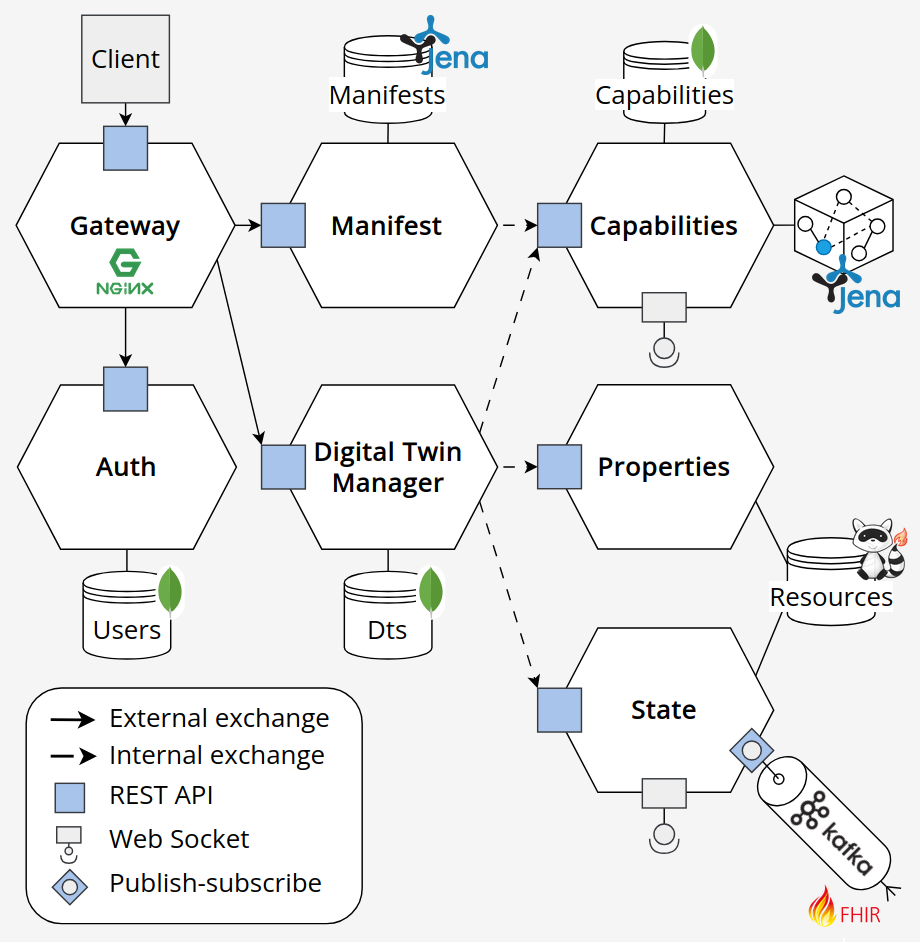
\includegraphics[width=1\linewidth]{figures/paper6/fig2.png}
    \caption{Micro-services architecture of the Digital Twin Layer.}\label{paper6_fig2}
\end{figure}

The domain modeling phase was notably time-intensive due to the heterogeneity of concepts across the various services. The Manifests uploaded are transformed into RDF graphs via the Jena RDF API and stored on a Fuseki server. We leveraged the FHIR specification to model the information describing the patient DT. Specifically, the FHIR Patient resource represents the Properties acting as the root linking all other standard resources (Observation, Encounter, etc.), modeling the State. The HAPI FHIR library facilitates development by providing a comprehensive Java implementation of the FHIR standard along with other utilities, including a client for effective interaction with FHIR-compliant services.

The system employs synchronous, blocking communication for both internal and external interactions, with a few key exceptions. In the Source Layer, data from external services and devices is converted into events and published to a Kafka event bus for asynchronous processing. Additionally, WebSockets enable real-time communication to exchange simulation results and monitor the state evolution of the DT.
%
%%%% CHANGED:
% \section{AI Model Semantic Binding via the Manifest Protocol}
%%%% TO:
\subsection{Manifest Protocol}\label{sec:paper6_manifest_protocol}
In CONNECTED, each DT can expose unique capabilities to predict future patient trajectories. These capabilities are underpinned by general-purpose AI models tailored to specific patient characteristics, which are activated upon triggering. Our framework seamlessly integrates the models through the Manifest protocol and automates all the crucial steps behind the execution of a DT capability: (1) takes a snapshot of the patient state and converts it into a KG; (2) retrieve the Manifest associated to that capability; (3) checks if the model interface can be fulfilled with the extracted data; (4) accesses and executes the models returning the result as soon as available.

%%%% CHANGED:
%%%% TO:
To evaluate the Manifest protocol, we selected a Neural Network classifier for stroke prediction originally proposed by Dev et al.~\cite{dev_predictive_2022}. We wrapped the model in Python, deployed it through a Flask web service, and independently recalculated its key performance metrics, including precision, recall, F1-Score, accuracy, miss rate, and false positive rate. Model validity was confirmed by ensuring that its accuracy fell within the distribution range reported by the authors. We then defined a Manifest instance describing the model's input requirements and registered it within CONNECTED. This enabled fully automated execution of the model via the Capabilities service. The metrics derived from Manifest-driven execution were compared with those from the baseline to confirm functional equivalence.

To further demonstrate the model-agnostic nature of the Manifest protocol, we also integrated a Decision Tree and Random Forest classifiers from Dev et al.'s study~\cite{dev_predictive_2022}. A dedicated Manifest instance was created for each model and uploaded within the infrastructure. These Manifests were then used to develop a proof-of-concept benchmarking application leveraging the framework’s RESTful APIs. This application showcases the semantic generality and technical flexibility of the Manifest protocol, which supports AI models regardless of their internal logic or complexity and validates the expressiveness of the CONNECTED API.

The Manifest protocol offers a level of automation that alleviates the technical burden on users, enabling them to concentrate on insight-driven decision-making. Its development required two distinct efforts: (a) the MIMO ontology to describe the AI models' interfaces, and (b) the implementation of the DT Capabilities component. 
%%%% CHANGED:
%%%% TO:
\subsubsection{MIMO: Design and Publication}
MIMO was designed following the Noy and McGuinness 1O1 Development Guide~\cite{mcguninnes}, and then implemented using the Protégé editor. It functions as a task ontology, capturing structural and operational aspects of executable models. It formally defines their interfaces as a combination of metadata, such as inputs, outputs, and location. We publicly released the MIMO ontology as a generalizable specification into the LOD repository to support reproducibility and promote reuse. Moreover, we documented MIMO using LODE (Live OWL Documentation Environment), a tool that automatically extracts ontology entities and generates human-readable HTML documentation based on their metadata \footnote{\url{https://model-interface-manifest-ontology-ad0613.gitlab.io/}}. Finally, the ontology was validated leveraging KGHeartBeat, an open-source KG quality assessment tool.
%%%% CHANGED:
%%%% TO:
\subsubsection{Semantic Binding and Orchestration}
The Capabilities component is realized as a dedicated microservice responsible for orchestrating model execution. When a specific capability is invoked, the service retrieves the required patient data and the corresponding model manifest by querying RESTful APIs exposed by the other services. These data sources are transformed into RDF-based KGs using the Jena RDF API and dynamically loaded into an in-memory graph at runtime.

A Jena reasoner, configured with OWL Description Logic (DL) rules and the Simulation and Integration Model Ontology (SIMO), is then applied to perform semantic inference. SIMO serves as a bridge between the model-centric MIMO schema and FHIR-compliant patient data representations. Notably, SIMO has not been published, as it is a task-specific application ontology developed to implement internal integration logics that are not intended for reuse beyond this context. The reasoner infers correspondences between a model’s input parameters and the patient data. Once valid mappings are established for all required inputs, the Capabilities service automatically triggers execution of the associated predictive model.

%%%% CHANGED:
%To evaluate the Manifest protocol, we selected a Neural Network classifier for stroke prediction originally proposed by Dev et al.~\cite{dev_predictive_2022}. We wrapped the model in Python, deployed it through a Flask web service, and independently recalculated its key performance metrics, including precision, recall, F1-score, accuracy, miss rate, and fall-out rate. Model validity was confirmed by ensuring that its accuracy fell within the distribution range reported by the authors. We then defined a Manifest instance describing the model's input requirements and registered it within CONNECTED. This enabled fully automated execution of the model via the Capabilities service. The metrics derived from Manifest-driven execution were compared with those from the baseline to confirm functional equivalence.
%
%To further demonstrate the model-agnostic nature of the Manifest protocol, we also integrated a Decision Tree and Random Forest classifiers from Dev et al.'s study~\cite{dev_predictive_2022}. A dedicated Manifest instance was created for each model and uploaded within the infrastructure. These Manifests were then used to develop a proof-of-concept benchmarking application leveraging the framework’s RESTful APIs. This application highlights the Manifest protocol's semantic generality and technical flexibility, which support AI models regardless of their internal logic or complexity, and validate the CONNECTED API's expressiveness.
%%%% TO:
%
\subsection{Evaluation and Experimental Results}~\label{sec:paper6_evaluation}
This section presents the principal outcomes of our work, structured around four core contributions: (1) the design and implementation of the DT Layer as a FHIR-compliant, patient-centric API enabling structured access to clinical history, real-time monitoring, and predictive simulation; (2) the development of the Model Interface Manifest Ontology (MIMO), published as LOD and evaluated through the HeartBeatKG quality assessment tool; (3) the validation of the Manifest protocol by integrating a well-established Neural Network model to identify patients at high risk of stroke; (4) the demonstration of the framework’s potential through a benchmarking proof-of-concept application that supports continuous evaluation of multiple stroke risk classifiers;
%%%% CHANGED: 
%%%% TO: 
and (5) a performance evaluation quantifying the platform’s scalability, latency, and throughput under concurrent workloads.
%%%% CHANGED:
% \subsection{Enabling Digital Twin Services through FHIR-Compliant API}
%%%% TO:
\subsubsection{FHIR-compliant API for DT Services}
Implementing CONNECTED opens new opportunities for healthcare applications by leveraging patient-specific DT to enhance clinical decision-making and streamline care delivery. 
%%%% CHANGED:
%%%% TO:
Unlike conventional systems that primarily provide raw data retrieval or event-based alerts, CONNECTED’s DTs offer a continuous, context-aware, and predictive representation of each patient. The platform’s FHIR-compliant REST API enables users to:
\begin{itemize}
    \item Retrieve comprehensive clinical histories, offering unified access to patient-centric, multi-source data.
    \item Monitor real-time health updates in the context of each patient’s evolving condition.
    \item Perform predictive simulations using integrated AI models, enabling clinicians to anticipate potential clinical trajectories.
\end{itemize}
%
This subsection illustrates these three core API-driven capabilities through UML sequence diagrams that reveal the system’s internal coordination. Each diagram focuses on the high-level orchestration among the framework's microservices, abstracting away lower-level infrastructure components such as authentication mechanisms, persistence layers, and proxy servers. The result is a clear and concise view of the logical information flow required to support each clinical use case.

\paragraph{Retrieving Patient Clinical History}
This operation allows external systems or applications to access a structured, comprehensive snapshot of a patient’s current and historical medical data. Specifically, the system returns a FHIR Bundle that encapsulates all relevant resources representing the patient's state at a given time. Figure~\ref{fig:paper6_clinical_history_sequence} illustrates that only the State service is required to fulfill the request.

% UML Sequence Diagram for Clinical History Retrieval
\begin{figure}
    \centering
    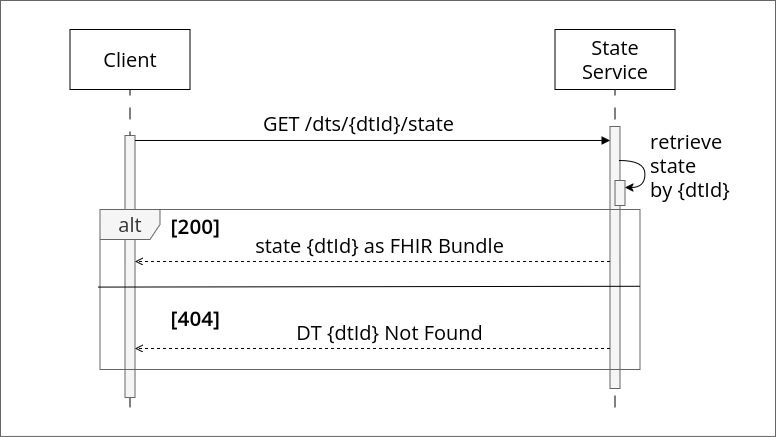
\includegraphics[width=1\linewidth]{figures/paper6/fig5.png}
    \caption{UML sequence diagram illustrating the patient’s clinical history retrieval request.}
    \label{fig:paper6_clinical_history_sequence}
\end{figure}

\paragraph{Real-time Monitoring of Patient Updates}
CONNECTED enables real-time patient monitoring by supporting continuous data streaming from each patient's DT to subscribed client applications. This capability is vital in dynamic clinical settings, where immediate access to the most current patient data is essential for timely and informed decision-making.

As depicted in Figure~\ref{fig:paper6_real_time_monitoring_sequence}, updates to the DT’s state are delivered via a persistent WebSocket connection and formatted in FHIR. Each state change is propagated as soon as it is registered within the system. For example, a medical device can trigger an update by publishing an event to the Kafka broker within the Source Layer. This event-driven architecture ensures low-latency data delivery and high responsiveness, facilitating seamless integration with real-time applications such as clinical dashboards, alerting mechanisms, and decision support systems.

\begin{figure}
    \centering
    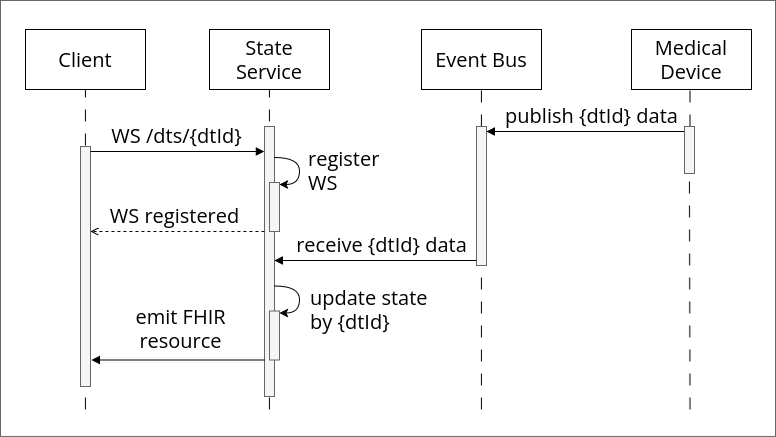
\includegraphics[width=1\linewidth]{figures/paper6/fig6.png}
    \caption{UML sequence diagram illustrating the patient real-time monitoring.}
    \label{fig:paper6_real_time_monitoring_sequence}
\end{figure}

\paragraph{Prediction of Patient Trajectories}
Among CONNECTED’s most advanced capabilities is its support for predictive simulations over patient-specific DTs by executing AI models defined via Manifests. This functionality empowers clinicians and healthcare applications to anticipate future clinical trajectories, such as the likelihood of disease onset or progression, based on a patient's most recent health status.

As shown in Figure~\ref{fig:paper6_predictive_trajectory_sequence}, a predictive request is initiated when the client application invokes a capability exposed by the patient’s DT. The platform then performs semantic alignment between the AI model’s input requirements specified in the Manifest and the current patient data encoded in the DT. If the necessary input parameters are available, CONNECTED automatically triggers the model execution through its dedicated API (labeled \texttt{Executable AI Model} in Figure~\ref{fig:paper6_predictive_trajectory_sequence}).

Given the potential computational cost of model inference, the framework executes prediction tasks asynchronously. Once the computation is completed, the prediction result is delivered back to the client via a WebSocket channel. This asynchronous design ensures non-blocking interactions, system scalability, and timely delivery of model outputs without compromising the user experience.

\begin{figure*}
    \centering
    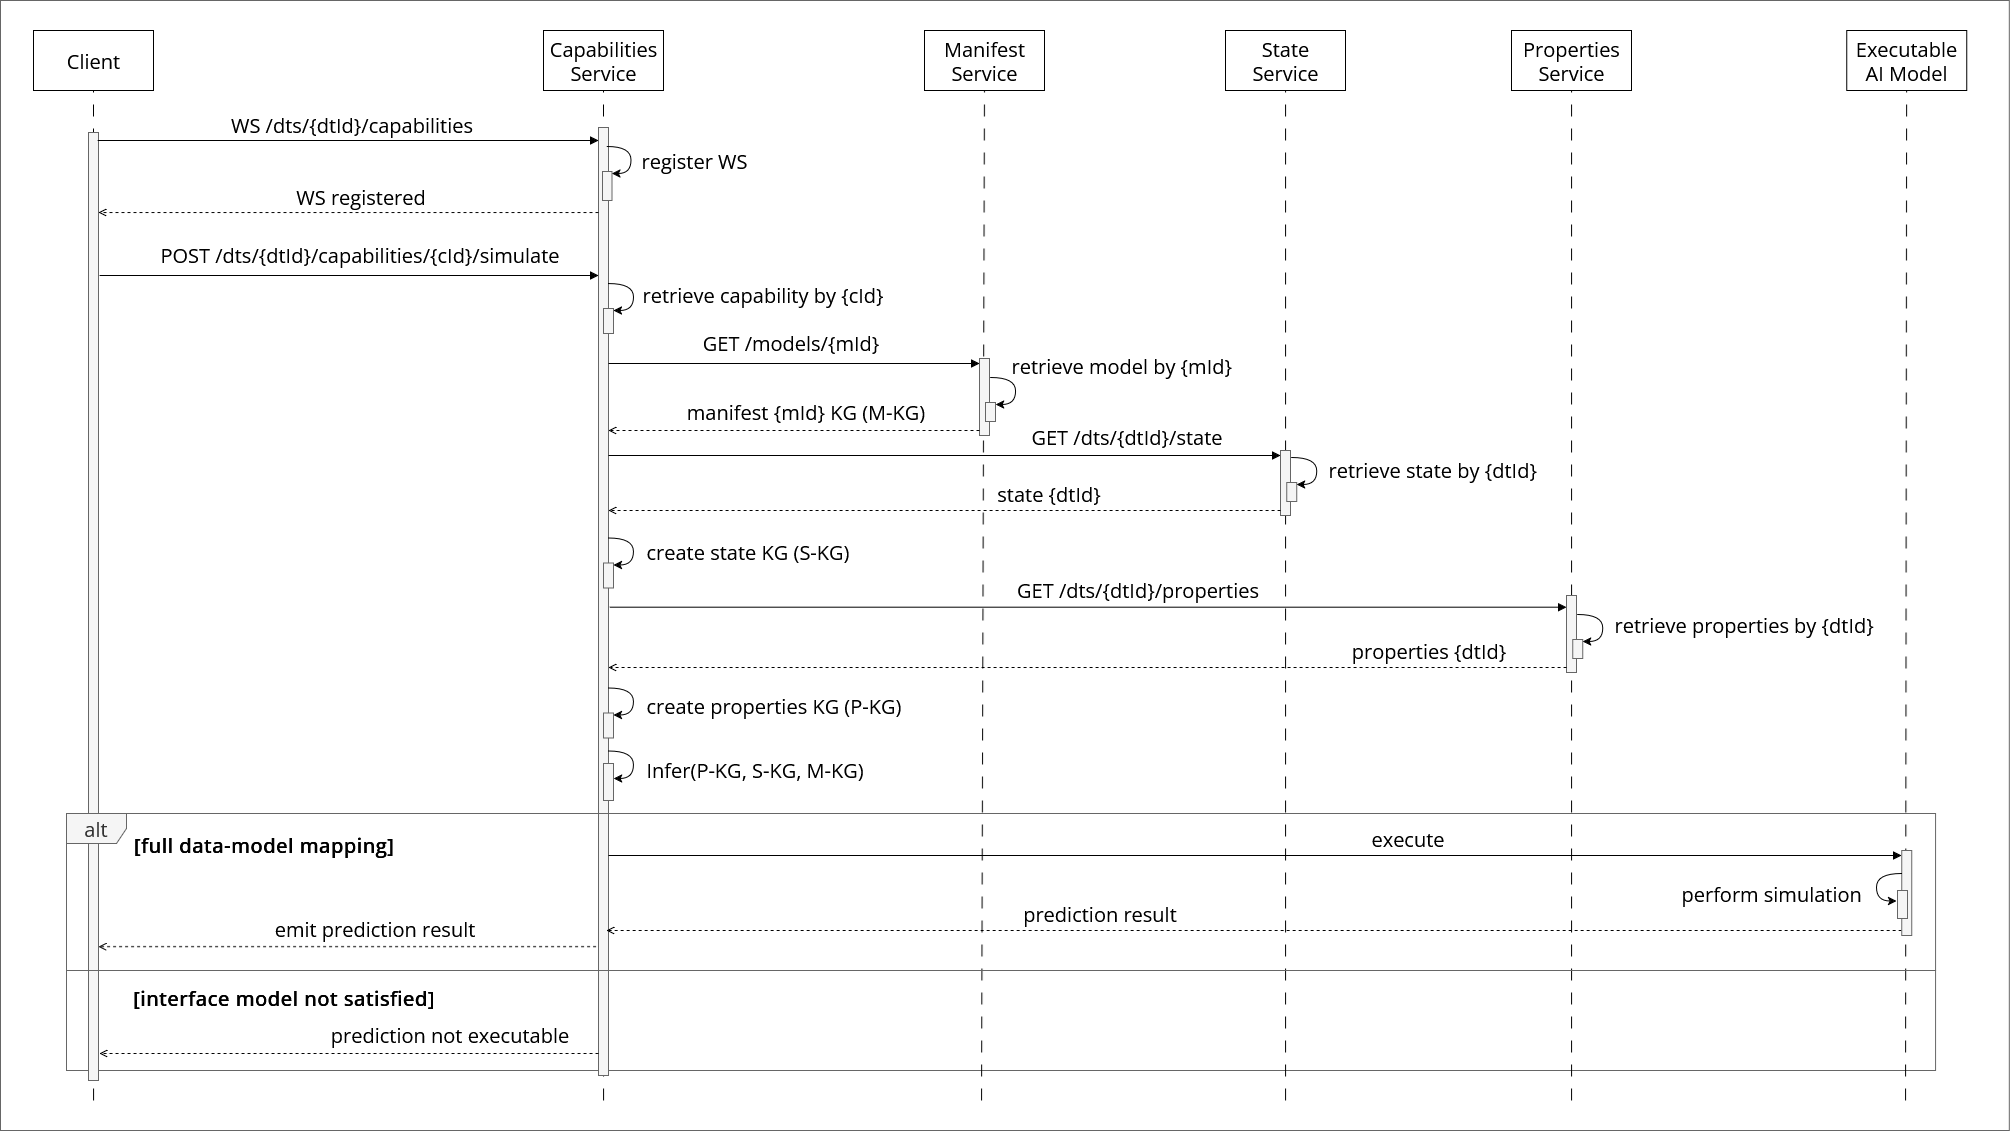
\includegraphics[width=1\linewidth]{figures/paper6/fig7.png}
    \caption{UML sequence diagram illustrating the prediction of future patient trajectories.}
    \label{fig:paper6_predictive_trajectory_sequence}
\end{figure*}

\subsubsection{MIMO: Ontology Quality Assessment}
MIMO was developed to formalize and support semantic descriptions of AI models for automated integration within DT architectures. The ontology was encoded in both OWL/XML (\texttt{.owl}) and Turtle (\texttt{.ttl}) serializations and is publicly available via our repository\footnote{\url{https://gitlab.com/unibo-connected/model-interface-manifest-ontology}}. It has also been published in the LOD\footnote{\url{https://lod-cloud.net/dataset/CONNECTED}}, ensuring discoverability, reuse, and interoperability across the semantic web ecosystem. The final release includes approximately 13 classes, 12 object properties, 8 data properties, and 65 logical axioms. The core foundational version contained 278 elements.

Figure~\ref{paper6_fig3} illustrates the core conceptual structure of MIMO, including its integration of Dublin Core annotation properties. These design choices enrich the ontology with standardized metadata and enhance semantic expressiveness.

\begin{figure}
    \centering
    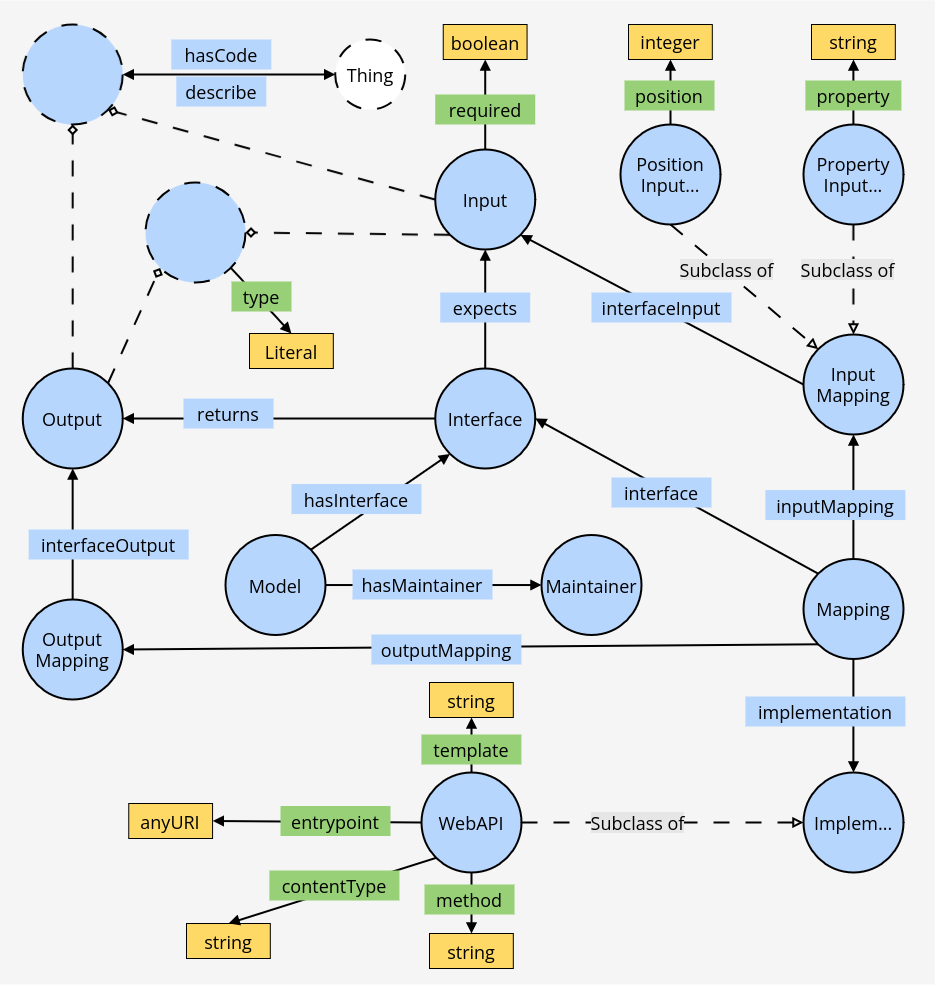
\includegraphics[width=1\linewidth]{figures/paper6/fig3.png}
    %%%% CHANGED: \caption{Visualization of the abstraction for the Model Interface Manifest Ontology.}\label{fig3}
    %%%% TO:
    \caption{MIMO ontology diagram illustrating OWL classes (blue circles), object properties (blue labels), and data properties (green labels), showing relationships among domain concepts. The ontology can be explored via \href{https://service.tib.eu/webvowl/\#iri=https://model-interface-manifest-ontology-ad0613.gitlab.io/MIMO.owl}{WebVOWL}.}\label{paper6_fig3}
\end{figure}

Logical validation was conducted using the Pellet Reasoner Plug-in (v2.2.0) within the Protégé environment. The reasoning process revealed no inconsistencies, affirming the ontology’s logical soundness and internal coherence. Furthermore, to evaluate MIMO's quality, we employed KGHeartBeat~\cite{pellegrino_kgheartbeat_2025}, a fully automated framework for KG quality assessment. It utilizes the \textit{Weighted Dimension Value} approach~\cite{debattista_luzzumethodology_2016} to produce normalized scores (0--100) across a broad spectrum of quality dimensions.
This methodology facilitates both fine-grained evaluation and holistic comparison.

The evaluation framework is grounded in the model proposed by Zaveri et al.~\cite{zaveri_2015}, which organizes quality assessment into 20 distinct dimensions, grouped under six dimension clusters:
\begin{itemize}
    \item \textit{Accessibility}: Pertains to data availability, licensing, interlinking, security, and performance aspects, all critical for reliable and authorized access.
    \item \textit{Intrinsic}: Focuses on context-independent features such as semantic accuracy, consistency, and conciseness, ensuring syntactic and logical integrity.
    \item \textit{Contextual}: Encompasses task-dependent metrics, with sub-clusters including:
    \begin{itemize}
        \item \textit{Trust}: Measures believability, reputation, and verifiability.
        \item \textit{Dataset Dynamicity}: Addresses temporal aspects such as currency and timeliness.
    \end{itemize}
    \item \textit{Representational}: Assesses the design and usability of data structures, including representational conciseness, interoperability, interpretability, understandability, and versatility.
\end{itemize}
%
Table~\ref{tab:paper6_qualitymetrics} presents the quality scores for each dimension. MIMO achieved a normalized total score of 71.3/100, indicating a high-quality design, particularly in the \textit{Intrinsic} and \textit{Representational} categories, essential for semantic interoperability and the seamless integration of AI components.

The table shows zero scores for metrics assessing links between MIMO and other ontologies. This applies to the Interlinking score, which evaluates alignment with other KGs; the Reputation score, derived from the PageRank algorithm to measure how many external graphs link to MIMO; and the Completeness score, which represents the ratio between triples with external links and the total triples of MIMO. This is because it is the first version of the ontology, which initially needs to support the integration of models into the platform. This basic operability is achieved without link MIMO to external knowledge graphs.

\begin{table}[ht]
\centering
%%%% CHANGED:
% \caption{KGHeartBeat Quality Metrics for MIMO by Dimension (Normalized 0--100)}
%%%% TO:
\caption{MIMO ontology quality scores computed with KGHeartBeat~\cite{pellegrino_kgheartbeat_2025}, following the methodology described in the \href{https://isislab-unisa.github.io/KGHeartBeat/}{official documentation}.}
\label{tab:paper6_qualitymetrics}
\begin{tabular*}{\tblwidth}{@{}LLC@{}}
\toprule
\textbf{Macro-group} & \textbf{Quality Dimension} & \textbf{Score} \\
\midrule
\multirow{5}{*}{Accessibility} 
  & Availability & 0.95 \\
  & Licensing & 1.00 \\
  & Interlinking & 0.00 \\
  & Security & 0.50 \\
  & Performance & 1.00 \\
\midrule
\multirow{3}{*}{Intrinsic} 
  & Semantic Accuracy & 1.00 \\
  & Consistency & 0.51 \\
  & Conciseness & 0.99 \\
\midrule
\multirow{3}{*}{Trust} 
  & Reputation & 0.00 \\
  & Believability & 0.75 \\
  & Verifiability & 0.99 \\
\midrule
\multirow{2}{*}{Dataset Dynamicity} 
  & Currency & 1.00 \\
  & Timeliness & 1.00 \\
\midrule
\multirow{2}{*}{Contextual} 
  & Completeness & 0.00 \\
  & Amount of Data & 1.00 \\
\midrule
\multirow{5}{*}{Representational} 
  & Representational Conciseness & 0.50 \\
  & Interoperability & 0.99\\
  & Understandability & 0.05  \\
  & Interpretability & 1.00 \\
  & Versatility & 1.00 \\
\midrule
\multicolumn{2}{l}{\textbf{Total Quality Score}} & \textbf{71.3} \\
\bottomrule
\end{tabular*}
\end{table}

%%%% CHANGED:
%\subsection{Test Manifest Protocol: Identifying High-risk Stroke Patients}
%%%% TO:
\subsubsection{Use Case: Stroke Risk Prediction}
A core innovation of the CONNECTED framework is its Manifest protocol. It enhances DTs with predictive capabilities through AI model integration. This protocol facilitates the seamless adaptation of general-purpose models to individual patients by incorporating historical and real-time clinical data. As a result, DTs can perform context-aware simulations with minimal manual configuration.

To test this mechanism, we implemented a use case focused on identifying patients at high risk of stroke. We integrated a Neural Network developed by Dev et al.~\cite{dev_predictive_2022}. It classifies stroke risk based on four key clinical features: age, average glucose level, hypertension status, and heart disease. The model was trained and evaluated using the dataset published in their public GitHub repository\footnote{\url{https://github.com/Soumyabrata/EHR-features}}, which includes 1,096 records—balanced between 548 stroke-positive and 548 stroke-negative patients. Following the original study, the dataset was split into training and testing sets using a 70:30 ratio, resulting in 329 test samples for performance evaluation.

We integrated the Neural Network within CONNECTED by defining a dedicated Manifest describing its structure, inputs, and expected outputs. This enabled its automated invocation via the Capabilities service, with patient data dynamically matched to the model’s input requirements. The resulting classification metrics from the Manifest-driven execution were compared against the original implementation to assess functional equivalence. The experimental setup and performance outcomes are detailed in the subsequent sections.

We follow the spirit of reproducible research, and therefore the created manifests, the models, and the code developed to realize this test and the proof-of-concept are available online\footnote{\url{https://gitlab.com/unibo-connected/connected-test}}.

\paragraph{Setup}
A total of 329 patients from the stroke classifier dataset~\cite{dev_predictive_2022} were used for simulation. For each patient, a DT was instantiated within the framework and populated with FHIR-based resources representing the four input features required by the model. These resources were further enriched with semantic annotations, including ontology references from standards such as LOINC and SNOMED-CT.

A Manifest describing the Neural Network was defined according to the MIMO ontology. This specification includes the model’s input parameters, API endpoint, expected data format, and execution constraints. The Manifest was uploaded to CONNECTED via the Manifest service and programmatically linked to the relevant DTs using the Capabilities service. Leveraging the framework’s data-to-model mechanism, all 329 DTs were automatically enhanced with stroke risk prediction capabilities.
%
\paragraph{Data Fusion and Semantic Integration}
For each DT, stroke risk prediction was initiated by invoking its associated capability. This process succeeds only if the DT contains sufficient data to satisfy the model’s input requirements: age, average glucose level, hypertension status, and heart disease. CONNECTED performs this validation automatically by extracting and combining three KGs: the Manifest, the Properties, and the current State of the DT. These graphs are then merged with domain ontologies (FHIR, MIMO, and SIMO) and passed to a Jena reasoner for semantic inference.

As illustrated in Figure~\ref{paper6_fig4}, the reasoner applies OWL-based description logic rules to infer semantic correspondences. Specifically, it establishes \texttt{canBeFulfilled} relationships between model input requirements and patient data nodes. The capability is deemed executable when the reasoner infers at least a link for each input.
%
\begin{figure*}
\centerline{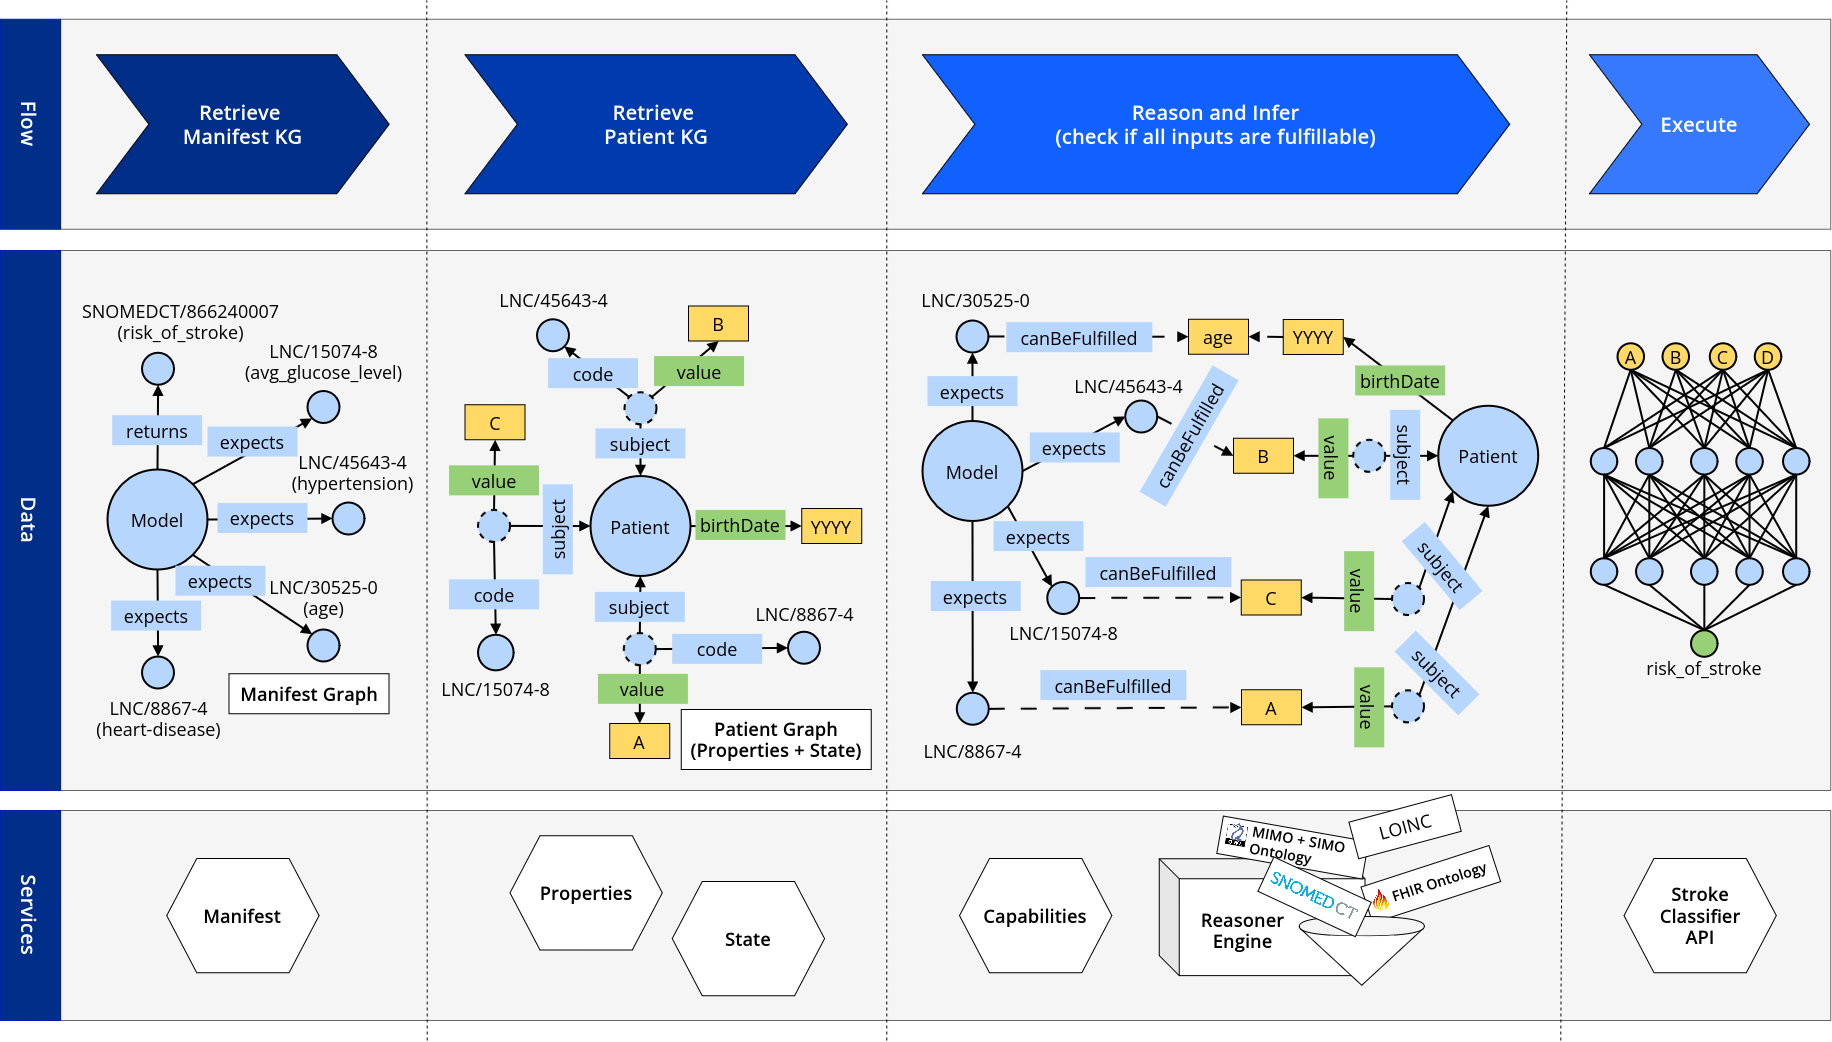
\includegraphics[width=\linewidth]{figures/paper6/fig4.png}}
\caption{Overview of the reasoning process aligning patient data with the stroke risk classifier’s input requirements.}
\label{paper6_fig4}
\end{figure*}
%
\paragraph{Simulation and Results Delivery}
As expected, CONNECTED’s internal data-model binding process matched all model inputs with corresponding patient information. Upon completion of semantic reasoning, the platform triggered the ML model by sending a properly formatted request to its API, as specified in the Manifest. The model’s binary prediction—indicating stroke risk—was then returned asynchronously via a WebSocket interface to the client application.

To validate correct integration, we compared the stroke risk predictions produced through Manifest-driven execution within CONNECTED against those generated by the original standalone Neural Network. Table~\ref{tab:paper6_model_comparison} shows that the evaluation metrics were identical across implementations. This confirms functional equivalence and demonstrates that the reasoning process does not introduce distortion or loss in predictive performance.

\begin{table}[ht]
\centering
\caption{Comparison of Neural Network performance metrics between standalone implementation and Manifest-driven execution in CONNECTED}
\label{tab:paper6_model_comparison}
\begin{tabular*}{\tblwidth}{@{}LCC@{}}
\toprule
\textbf{Metric} & \textbf{Standalone NN} & \textbf{CONNECTED Execution} \\
\midrule
Precision       & 0.74 & 0.74 \\
Recall          & 0.85 & 0.85 \\
F1-Score        & 0.79 & 0.79 \\
Accuracy        & 0.78 & 0.78 \\
Miss Rate       & 0.09 & 0.09 \\
Fall-out Rate   & 0.30 & 0.30 \\
\bottomrule
\end{tabular*}
\end{table}

%This highlights DT platforms’ potential to deliver personalized insights, identify high-risk patients, and support clinical decision-making. By integrating ML models, CONNECTED establishes a scalable approach for predictive healthcare, paving the way for diverse future applications.

%%%% CHANGED:
%\subsection{Application Use Case: A Proof-of-Concept for Model Benchmarking}
%%%% TO:
\subsubsection{Proof-of-Concept Benchmarking Application}
To further demonstrate the model-agnostic capabilities of the Manifest protocol and the practical utility of CONNECTED, we developed a proof-of-concept benchmarking application located at the Application Layer of the architecture. This application interacts with DTs via the framework's RESTful APIs and illustrates how diverse AI models can be semantically integrated, invoked, and evaluated through a uniform interface.

In this use case, we incorporated two additional stroke classifiers—Random Forest and Decision Tree—from Dev et al.’s study~\cite{dev_predictive_2022}, alongside the previously validated Neural Network. Each model was described using a distinct Manifest, detailing its input requirements, API endpoint, and constraints according to the MIMO ontology. These Manifests were uploaded to CONNECTED and linked to the DTs as new executable capabilities.

%%%% CHANGED:
%We designed an incremental evaluation strategy to emulate the gradual accumulation of data in real-world deployments. The 329 test patients were partitioned into ten sequential subsets (or “chunks”), progressively expanding the evaluation set by 10\% increments at each stage (e.g., 10\%, 20\%, ..., 100\%). Importantly, the models were not retrained or fine-tuned during this process; they remained static, enabling us to observe how their pretrained performance generalizes as new patient data is introduced. Specifically, we computed standard classification metrics (accuracy, precision, recall, and F1-score) after each evaluation set expansion. 

%This evaluation highlights not only static performance but also the robustness of each model, which is essential in clinical settings where decisions must often be made with limited initial data. As shown in Table~\ref{tab:benchmarking-metrics} and illustrated in Figure~\ref{fig:benchmarking-results}, performance variability is more pronounced in the early stages due to limited sample sizes. However, metrics stabilize as more patient data is incorporated, revealing each model’s robustness under evolving data conditions. Once stabilized, the Neural Network consistently achieved the highest performance among the tested models, confirming prior findings reported in Dev et al.~\cite{dev_predictive_2022}.
%%%% TO:
We designed an incremental evaluation strategy to emulate the gradual accumulation of patients in real-world deployments. In this work a test patient denotes a full patient-level record containing all available information for a single individual (demographics and the clinical features required by the models). The 329 patient-level records were partitioned into ten non-overlapping subsets (chunks) and the models were evaluated on the cumulative union of these chunks: stage $k$ uses the first $k$ chunks (10\%, 20\%, \dots, 100\% of the patients). Chunking was performed via stratified sampling to preserve the original stroke / non-stroke class ratio in each chunk, and the split is deterministic (fixed random seed) to ensure reproducibility. Chunk sizes are 33 patients for chunks 1–9 and 32 patients for chunk 10 (total 329). Importantly, models were kept static (no retraining or fine-tuning) between stages so that each stage measures how pretrained models generalize as new, distinct patients are introduced.

This incremental evaluation highlights not only static performance but also model robustness when operating with limited cohorts—an important property in clinical settings where decisions are often required early in deployment. After each cumulative expansion we computed standard classification metrics (accuracy, precision, recall, and F1-score) and report mean and dispersion (standard deviation and 95\% confidence intervals) across repeated runs. As shown in Table~\ref{tab:paper6_benchmarking-metrics} and Figure~\ref{fig:paper6_benchmarking-results}, performance variability is larger in early stages due to small sample sizes and stabilizes as more patient-level records are incorporated; once stabilized, the Neural Network consistently attains the highest performance among the tested models, in agreement with Dev et al.~\cite{dev_predictive_2022}. 

\begin{table*}[ht]
\centering
%%%% CHANGED:   
% \caption{Incremental evaluation of model performance over 10 cumulative patient data chunks. Metrics: Accuracy, Precision, Recall, and F1-score, reported for Neural Network (NN), Random Forest (RF), and Decision Tree (DT).}
%%%% TO:
\caption{Accuracy trends for Neural Network (NN), Random Forest (RF), and Decision Tree (DT) evaluated on cumulative patient-level test sets. The 329 patient-level records were partitioned into ten non-overlapping, stratified chunks.}
\label{tab:paper6_benchmarking-metrics}
\renewcommand{\arraystretch}{1.2}
\resizebox{\textwidth}{!}{% layout: resized to the thesis text width
\begin{tabular}{|c|c|ccc|ccc|ccc|ccc|}
\hline
\multirow{2}{*}{\textbf{Chunk}} & \multirow{2}{*}{\textbf{N}} & \multicolumn{3}{c|}{\textbf{Accuracy}} & \multicolumn{3}{c|}{\textbf{Precision}} & \multicolumn{3}{c|}{\textbf{Recall}} & \multicolumn{3}{c|}{\textbf{F1-score}} \\
\cline{3-14}
 &  & \textbf{NN} & \textbf{RF} & \textbf{DT} & \textbf{NN} & \textbf{RF} & \textbf{DT} & \textbf{NN} & \textbf{RF} & \textbf{DT} & \textbf{NN} & \textbf{RF} & \textbf{DT} \\
\hline
1  & 33  & 0.76 & 0.82 & 0.70 & 0.78 & 0.89 & 0.79 & 0.86 & 0.81 & 0.71 & 0.82 & 0.85 & 0.75 \\
2  & 66  & 0.77 & 0.79 & 0.71 & 0.78 & 0.84 & 0.78 & 0.88 & 0.80 & 0.72 & 0.82 & 0.82 & 0.75 \\
3  & 99  & 0.79 & 0.76 & 0.69 & 0.78 & 0.81 & 0.74 & 0.88 & 0.75 & 0.70 & 0.82 & 0.78 & 0.72 \\
4  & 132 & 0.80 & 0.73 & 0.68 & 0.81 & 0.80 & 0.76 & 0.86 & 0.73 & 0.68 & 0.83 & 0.77 & 0.72 \\
5  & 165 & 0.79 & 0.75 & 0.67 & 0.78 & 0.78 & 0.72 & 0.87 & 0.73 & 0.64 & 0.82 & 0.76 & 0.68 \\
6  & 198 & 0.79 & 0.74 & 0.67 & 0.75 & 0.76 & 0.69 & 0.87 & 0.73 & 0.62 & 0.81 & 0.74 & 0.66 \\
7  & 231 & 0.79 & 0.75 & 0.67 & 0.77 & 0.78 & 0.70 & 0.87 & 0.74 & 0.63 & 0.81 & 0.76 & 0.66 \\
8  & 264 & 0.78 & 0.75 & 0.66 & 0.75 & 0.75 & 0.68 & 0.85 & 0.76 & 0.64 & 0.80 & 0.75 & 0.66 \\
9  & 296 & 0.78 & 0.74 & 0.66 & 0.74 & 0.73 & 0.67 & 0.85 & 0.75 & 0.64 & 0.79 & 0.74 & 0.66 \\
10 & 329 & 0.78 & 0.74 & 0.66 & 0.74 & 0.73 & 0.66 & 0.85 & 0.76 & 0.65 & 0.79 & 0.74 & 0.66 \\
\hline
\end{tabular}
}
\end{table*}

\begin{figure}
\centerline{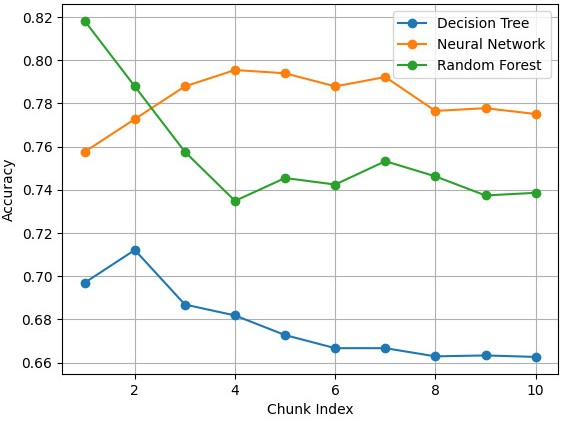
\includegraphics[width=\linewidth]{figures/paper6/fig8.jpeg}}
%%%% CHANGED:
% \caption{Accuracy trends for Neural Network, Decision Tree, and Random Forest models as the evaluation set incrementally increases.}
%%%% TO:
\caption{Accuracy trends for Decision Tree (DT), Neural Network (NN), and Random Forest (RF) as the evaluation set grows. Each point is computed on a cumulative patient-level set formed by sequentially adding non-overlapping patient groups (stage~1: $\approx$33 patients; stage~10: 329).}
\label{fig:paper6_benchmarking-results}
\end{figure}

Beyond benchmarking, this experiment underscores a broader capability of the framework: acting as a dynamic, semantically harmonized repository of patient-specific data. By continuously aggregating up-to-date clinical information into structured FHIR-based representations, CONNECTED enables ongoing validation of AI models under realistic and evolving conditions. As healthcare data streams from diverse sources, the system can support longitudinal model assessments, detect performance drift, and assist in model lifecycle monitoring—crucial elements for deploying safe and reliable AI in healthcare.

Moreover, the framework's semantic mediation and Manifest-driven execution architecture ensure that models can be assessed uniformly, regardless of their internal implementation or origin. This decoupling of models from data infrastructure reinforces CONNECTED's role as a testbed for adaptive deployment strategies in clinical environments.
%
%%%% CHANGED:
%%%% TO:
\subsubsection{Performance Evaluation}\label{sec:paper6_performance}
This section evaluates the performance of the CONNECTED platform in terms of scalability, latency, and throughput under varying levels of concurrent load. The aim is to provide concrete evidence of the platform's computational footprint and responsiveness in realistic deployment conditions, identify likely bottlenecks, and offer guidance on minimum and recommended system requirements for small- to medium-scale use.

All experiments were executed on a single-host deployment running the full CONNECTED application stack inside Docker containers. The host machine used for the experiments was equipped with an AMD Ryzen~5~5600X (6 physical cores), 16\,GB of RAM, and Ubuntu~24.04~LTS; Docker~24.0+ and Docker~Compose~2.20+ were used to orchestrate the containers, and Python~3.10+ was used for benchmarking. To inform prospective adopters, we recommend a minimum baseline configuration of a 4-core CPU, 8\,GB RAM, and 10\,GB of available disk for modest, single-host deployments; for moderate production usage, we recommend a 6-core CPU and 16\,GB RAM (the configuration used in our tests). During the heaviest tested load (20 concurrent threads), the host’s average memory consumption was approximately 2.8\,GB, indicating a modest memory footprint for the evaluated scenario.

Workload generation and measurement were performed using a custom Python profiling script that employs a \texttt{ThreadPoolExecutor} to issue concurrent HTTP prediction requests against the platform’s REST API. Each request executed a complete digital-twin simulation for a single patient and returned the corresponding prediction. Each experimental run issued 329 independent requests (matching the evaluation dataset); no caching or shared state was used between requests. We exercised four concurrency levels (1, 5, 10, and 20 worker threads) and collected per-request response traces from which we derived mean and median latency (ms), 95th-percentile latency (p95, ms), and throughput (successful requests per second, req/s).

Table~\ref{tab:paper6_performance} summarizes the measured metrics across all concurrency levels. As concurrency increases, overall throughput rises substantially, from 5.4\,req/s at a single thread to 26.7\,req/s at 20 threads. However, this improvement is accompanied by a gradual increase in latency: the mean latency grows from 185\,ms (1 thread) to 737\,ms (20 threads), and the 95th percentile latency reaches approximately 912\,ms.
\begin{table*}[ht]
\centering
\caption{Performance metrics across different concurrency levels.}
\label{tab:paper6_performance}
\resizebox{\textwidth}{!}{% layout: resized to the thesis text width
\begin{tabular}{c c c c c}
\toprule
\textbf{Concurrency} & \textbf{Mean (ms)} & \textbf{Median (ms)} & \textbf{p95 (ms)} & \textbf{Throughput (req/s)} \\
\midrule
1  & 184.98 & 182.05 & 204.11 & 5.41 \\
5  & 242.19 & 240.20 & 286.58 & 20.48 \\
10 & 385.98 & 382.64 & 467.93 & 25.70 \\
20 & 736.90 & 745.12 & 912.40 & 26.71 \\
\bottomrule
\end{tabular}
}
\end{table*}
%
Figure~\ref{fig:paper6_performance_plots} provides a visual summary of the performance behavior. The latency cumulative distribution (Figure~\ref{fig:paper6_latency_cdf}) shows that, in sequential execution, most requests complete within 200\,ms, indicating a low base latency under minimal contention. The throughput plot (Figure~\ref{fig:paper6_throughput}) highlights the scalability of the platform: throughput grows almost linearly up to 10 concurrent threads before plateauing near 26\,req/s. This behavior suggests that the system effectively utilizes available CPU cores up to a certain point, after which contention and scheduling overheads limit further gains. The 95th percentile latency (Figure~\ref{fig:paper6_p95_latency}) exhibits a similar pattern, increasing sharply beyond 10 threads due to resource competition among containers.
%
\begin{figure*}[t]
    \centering
    % Subfigure 1
    \begin{subfigure}{0.32\linewidth}
        \centering
        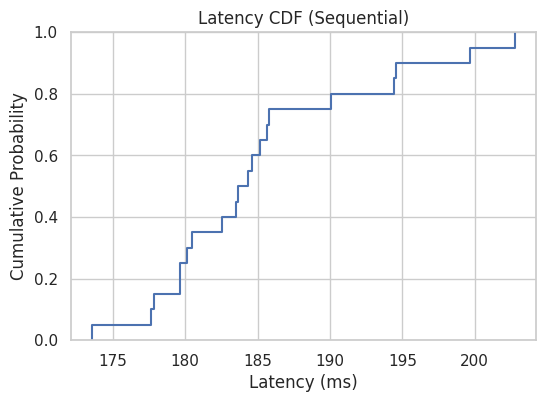
\includegraphics[width=\linewidth]{figures/paper6/fig9.png}
        \caption{Latency CDF (Sequential)}
        \label{fig:paper6_latency_cdf}
    \end{subfigure}
    \hfill
    % Subfigure 2
    \begin{subfigure}{0.32\linewidth}
        \centering
        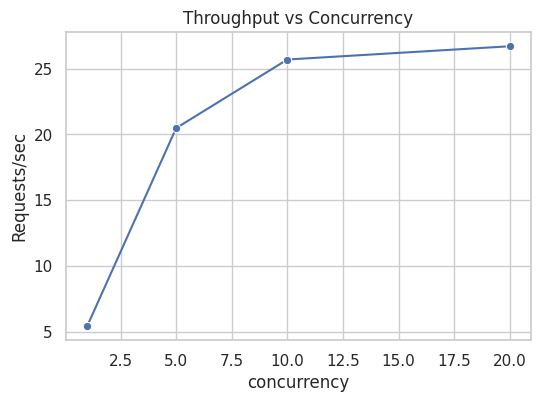
\includegraphics[width=\linewidth]{figures/paper6/fig10.png}
        \caption{Throughput vs Concurrency}
        \label{fig:paper6_throughput}
    \end{subfigure}
    \hfill
    % Subfigure 3
    \begin{subfigure}{0.32\linewidth}
        \centering
        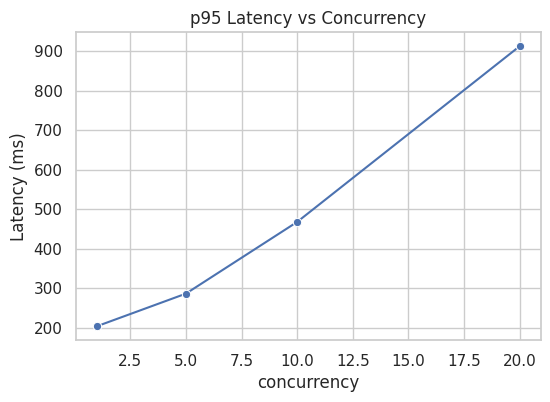
\includegraphics[width=\linewidth]{figures/paper6/fig11.png}
        \caption{95th Percentile Latency vs Concurrency}
        \label{fig:paper6_p95_latency}
    \end{subfigure}
    %
    \caption{
        Performance evaluation of the CONNECTED platform.
        (a) Cumulative distribution of request latency for sequential execution.
        (b) Throughput scaling with increasing concurrency levels.
        (c) Variation of the 95th percentile latency with concurrency.
    }
    \label{fig:paper6_performance_plots}
\end{figure*}
Overall, these results demonstrate that the CONNECTED platform scales efficiently up to moderate levels of concurrency while maintaining acceptable response times. The observed throughput–latency tradeoff is consistent with the expected behavior of containerized, compute-intensive workloads.
\subsection{Discussion}~\label{sec:paper6_discussion}
This work presented a preliminary implementation of the CONNECTED framework, demonstrating its effectiveness in supporting the deployment of semantically enriched, AI-powered DTs for healthcare applications. The platform is designed to predict future patient trajectories while promoting semantic interoperability, model transparency, and automation of model integration through Semantic Web technologies.

Our core contributions include: (1) the development of a FHIR-compliant, patient-centric API (DT Layer) that enables structured access to clinical histories, real-time health monitoring, and simulation of future states; (2) the publication of MIMO within the LOD Cloud, facilitating transparent, standards-based model interface descriptions; (3) the implementation of the Manifest protocol to automate data-to-model binding, thereby enabling seamless integration of AI models tailored to individual patient profiles; and (4) a proof-of-concept benchmarking application that continuously evaluates and ranks stroke risk classifiers in real time, driven by streaming patient data.

A key strength of CONNECTED lies in its modular, microservice-based architecture, which promotes scalability, flexibility, and ease of maintenance. The ability to dynamically integrate AI models through declarative manifests enables the system to adapt to new clinical domains and use cases. Furthermore, the semantic infrastructure powered by ontologies and KGs supports standardized model descriptions and rich patient representations, improving interpretability and reuse.
%
\subsubsection{Challenges and Limitations}
Despite its promise, the CONNECTED framework faces several limitations that must be addressed to achieve broader real-world applicability. First, the platform lacks substantial engagement from key stakeholders, including healthcare professionals, domain experts, and patients. This gap hinders the validation of its practical utility and the alignment of services with clinical needs. Moreover, its expressivity has been tested only within a controlled use case, limiting generalizability to diverse healthcare scenarios.

Technically, the current implementation of the Application Layer is emulated through a REST client and is not driven by end-user requirements. Future developments require stakeholder collaboration to design services that better meet clinical needs. Additionally, the platform's support for a patient-centered care model remains limited.

Privacy and security pose significant challenges, particularly given the sensitive nature of health data. Ensuring compliance with data protection regulations and implementing robust safeguards are imperative~\cite{jawad_security_2024}. Socio-ethical concerns—including algorithmic bias, legal uncertainties, and the high cost of implementation—also pose risks to adoption and may exacerbate existing disparities in healthcare delivery~\cite{Katsoulakis2024}.

From a systems perspective, the implemented framework assumes the availability of clean, reliable, and harmonized data from the Source Layer. This assumption is often unrealistic due to the heterogeneity and fragmentation of healthcare data systems. Furthermore, CONNECTED lacks a coherent strategy for historical data management, including decisions about long-term storage and appropriate technologies.

The platform employs a synchronous communication pattern that may become a bottleneck in high-throughput environments, raising scalability concerns. The platform also lacks well-defined authorization mechanisms (e.g., Role-Based Access Control), introducing potential security vulnerabilities. Additionally, the inability of individual Digital Twins to collaborate restricts the platform’s analytical potential, while the symbolic AI components, especially those facilitating explainability, are underutilized.

Finally, the assumption that each model independently handles data preprocessing can hinder integration, especially for models with stringent input requirements or dependencies.

\subsubsection{Future Research}
Future research will prioritize enhancing stakeholder engagement, technical scalability, and clinical usability. A clinician dashboard will be developed to support the orchestration and analysis of DTs, enabling users to manage patient profiles, simulate health trajectories over varying time frames, and compare predicted outcomes. Moreover, we will realize an intelligent assistant that interacts with individual patient twins to enhance engagement by offering proactive insights, alerts, and access to clinical histories.

On the technical front, robust and flexible data ingestion mechanisms are critical. This includes the adoption of communication middleware (e.g., Eclipse Hono) to support protocol translation, proprietary-to-FHIR mappings, and asynchronous data flows. Strategies like ETL pipelines, data aggregation, and distributed database replication will be explored to accommodate the growing volume of patient data.

The communication architecture should shift toward an asynchronous, event-driven model to support higher scalability and resilience. Establishing a standard workflow framework for data preprocessing will also be essential, enabling broader compatibility with diverse AI models. Additionally, enabling model pipelines—where the output of one model serves as input to another—will allow the definition of compound capabilities and support multi-stage analyses.

A pivotal direction for future work is the integration of Collective Digital Twins (CDTs), representing patient cohorts rather than individuals. This population-level abstraction will enable cohort-based analysis (e.g., filtering by age, diagnosis, or risk factors) and serve as a harmonized data source for training and validating AI models. This shift also introduces the opportunity to support model development, not just model deployment, thereby enabling the integration of MLOps principles into the CONNECTED pipeline.

The evolution of MIMO is central to this vision. It will be extended to describe model-related metadata such as performance metrics, training datasets, licensing terms, ethical considerations, and data sensitivity. To this end, we plan to align MIMO with the Model Card Report Ontology (MCRO)~\cite{Amith2022}, enhancing transparency and responsible AI practices.

An additional extension of MIMO will support the composition of model interfaces. Given formal descriptions of model inputs and outputs, it becomes feasible to orchestrate multi-model pipelines where intermediate outputs serve as inputs for subsequent models, thus enabling composite DT capabilities and more insightful analysis.

Finally, leveraging the patient-centric KG will further enrich CONNECTED's potential. The KG can be augmented via link prediction to infer missing relations and support reasoning over incomplete data. This future extension would also enhance explainability by connecting AI predictions to clinically accepted ontologies, offering interpretable pathways for decision support. In addition, the KG enables exploratory search, helping clinicians and researchers uncover hidden patterns and draw deeper insights from patient-specific data.

These research directions will reinforce CONNECTED’s role as a general-purpose framework for deploying AI-powered patient DTs. In particular, these extensions will enhance its adaptability to the evolving healthcare landscape, supporting the development of intelligent, insight-driven applications that respond to the dynamic needs of both patients and providers.

\subsection*{Code Availability}
The CONNECTED code is available from the corresponding author upon reasonable request. MIMO is publicly accessible in the LOD Cloud at \url{https://lod-cloud.net/dataset/CONNECTED}, with OWL documentation provided at \url{https://model-interface-manifest-ontology-ad0613.gitlab.io/}. All artifacts related to the Manifest protocol evaluation and the benchmarking proof-of-concept—including manifests, AI models, and supporting code—are openly available at: 
\url{https://gitlab.com/unibo-connected/connected-test}

\subsection*{Acknowledgment}
This study was partially supported by the Italian Ministry of University and Research under PNRR-PNC Project PNC0000002 ”DARE – Digital Lifelong Prevention” (CUP: B53C22006450001).

% layout: keep this paper's floats within its section
\FloatBarrier
